\documentclass[doc]{apa6}

\usepackage[english]{babel}
\usepackage[utf8x]{inputenc}
\usepackage{amsmath}
\usepackage{graphicx}
\usepackage{apacite}
\usepackage{amsfonts}
\usepackage{url}
\usepackage{tikz}
\usetikzlibrary{bayesnet}
\usepackage{subfigure}

%\usepackage[style=apa,sortcites=true,sorting=nyt,backend=biber]{biblatex}
%\DeclareLanguageMapping{american}{american-apa}

  \title{Supplemental Information: Warm (for Winter): Inferring comparison classes for scalar adjectives}
    \author{Michael Henry Tessler and Noah D. Goodman}
    \date{}
  
\shorttitle{ SI: Inferring comparison classes}
\affiliation{Stanford University}
\keywords{comparison class; pragmatics; Rational Speech Act; Bayesian cognitive model; Bayesian data analysis\newline\indent Word count: X}
\makeatletter
\newcommand\LastLTentrywidth{1em}
\newlength\longtablewidth
\setlength{\longtablewidth}{1in}
\usepackage{tabularx}
\usepackage{multicol}
\usepackage{wrapfig}
\usepackage{gensymb}
\usepackage{tikz}
\usepackage{caption}
\usepackage{booktabs}

\begin{document}
\maketitle

\definecolor{Red}{RGB}{255,0,0}
\definecolor{Green}{RGB}{10,200,100}
\definecolor{Blue}{RGB}{10,100,200}
\definecolor{Orange}{RGB}{255,153,0}

\newcommand{\denote}[1]{\mbox{ $[\![ #1 ]\!]$}}
\newcommand*\diff{\mathop{}\!\mathrm{d}}
\newcommand{\red}[1]{\textcolor{Red}{#1}}  
\newcommand{\ndg}[1]{\textcolor{Green}{[ndg: #1]}}  
\newcommand{\mht}[1]{\textcolor{Blue}{[mht: #1]}}  
\newcommand{\mlb}[1]{\textcolor{Orange}{[mlb: #1]}}

\section{Alternative Models}


\begin{figure}[t]
    \centering
    \subfigure[A literal model that does not represent a speaker's representation of the context as separate from their own. This listener effectively answers the question of what is more likely: a basketball player who is tall or a person who is tall?]{\label{fig:alternativeModelPredictions}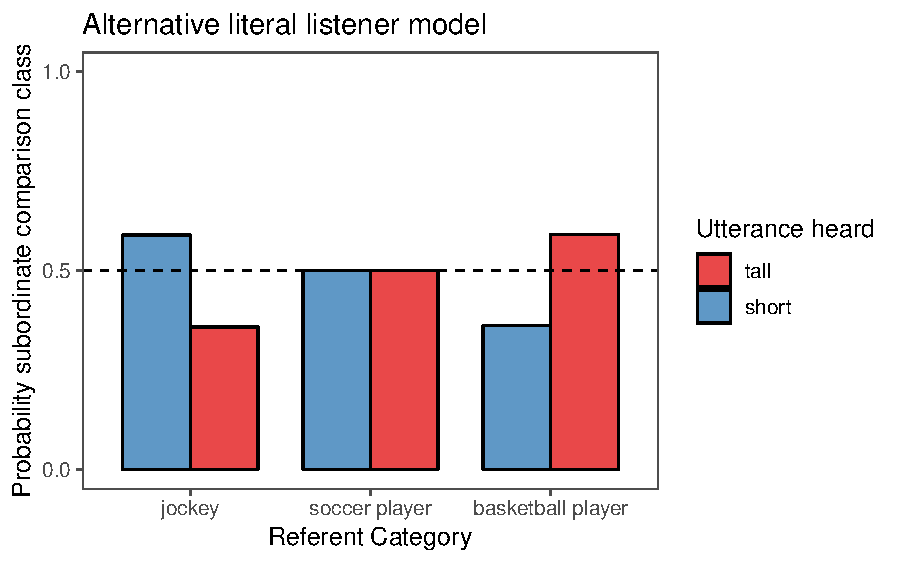
\includegraphics[width=0.48\textwidth]{figs/cc_inference_L0.pdf}}
    \subfigure[A more sophisticated pragmatic listener model that reasons about which comparison class a speaker believes that the listener would infer. ]{\label{fig:alternativeModelPredictions2}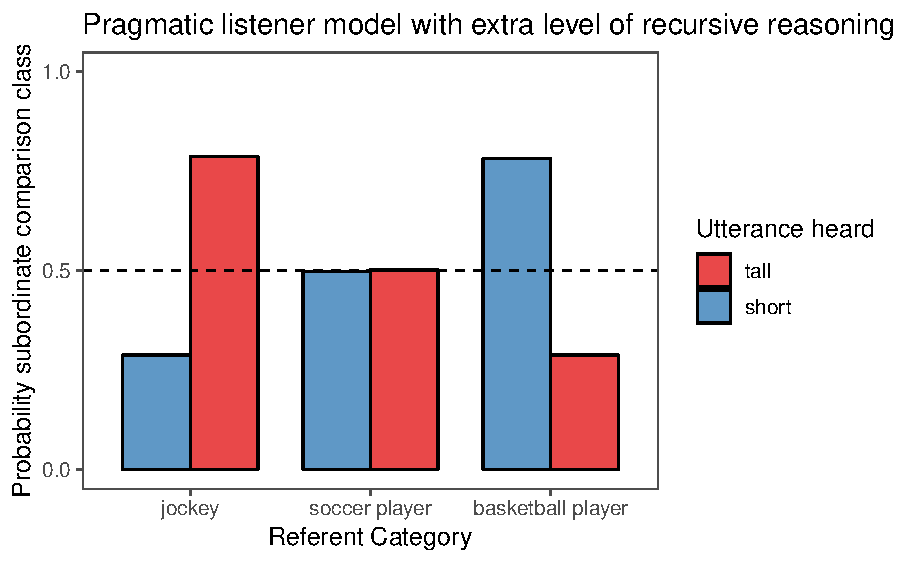
\includegraphics[width=0.48\textwidth]{figs/cc_inference_L2.pdf}}
    \caption{Alternative model predictions.}
\end{figure}


\subsection{Literal alternative model}

The inference about the comparison class outlined above involves a listener reasoning about a speaker reasoning about a listener.
One might wonder whether the inference about the comparison class is necessarily a pragmatic inference.
We can answer this question by reformulating the comparison class inference  spelled out in Equation \ref{eq:L1} in terms of a literal listener model (\emph{a la} Equation \ref{eq:L0}). 
This literal comparison class inference model is given by:
%
  \begin{align}
L_{0}(x, \theta, c \mid u, k) &\propto \delta_{[\![u]\!](x, \theta)} \cdot P(x \mid c) \cdot P(c \mid k) \cdot P(\theta) \label{eq:L0alt}
\end{align}
%
Similar to the pragmatic listener model (Eq.~\ref{eq:L1}), this listener can use their knowledge of the referent $k$ to constrain the hypothesis space of comparison classes (e.g., with the knowledge that the referent is a basketball player, consider comparison classes that the same as or superordinate to the class of basketball players).
Unlike the pragmatic listener model, however, the literal listener version of the model does not hold different representations of the referent in mind: The pragmatic listener has their private representation of the referent---given by the prior distribution of the degree $P(x \mid k)$---and imagines a speaker who acts assuming some comparison class---$S(u \mid c)$---where $c$ and $k$ may or may not index the same class (e.g., the listener knows the referent is a basketball player, but believes the speaker was assuming a \emph{person comparison class}).
The literal listener version of the model cannot separate these representations.
In effect, this listener is answering a slightly different question from the comparison class inference problem. The question this alternative model is answering is: what is more likely---a basketball player whose height is greater than some threshold or a person whose height is greater than some threshold? 
This alternative model predicts the exact opposite pattern of results from the pragmatic listener model (Figure \ref{fig:alternativeModelPredictions}). 

\subsection{Alternative pragmatic model}

The pragmatic comparison class inference listener model (Eq. \ref{eq:L1}) reasons about which comparison class a speaker is more likely to be assuming.
That is, the speaker (Eq. \ref{eq:S1}) is presumed to be assuming that a particular comparison class is already in the common ground, analogous to a presupposition (e.g., saying ``My car is in the shop'' presupposes that the speaker owns a car). 
Speakers may be aware, however, that the comparison class is not in the common ground, but may still avoid articulating a comparison class if the listener can reasonably be assumed to infer the comparison class. This kind of inference is more sophisticated: It involves a listener reasoning about the comparison class that a speaker believed  the listener would infer, given that the first-order listener inference about the comparison class itself involves a pragmatic inference. %\ndg{??:  as shown via counterexample by the literal model above}. 
This higher-order reasoning model is given by the following equations:

\begin{align}
L_2(x, c \mid u, k) &\propto S_2(u \mid x, c) \cdot P(x \mid k) \cdot P(c \mid k) \label{eq:L2} \\
S_2(u \mid x, c) &\propto \exp{(\alpha \cdot (\ln L_{1}(x, c \mid u) - \text{cost}(u) ))}\label{eq:S2} 
\end{align}

The primary difference between this model and the model given by Eqs.~\ref{eq:L1} and \ref{eq:S1} is in the speaker $S_2$.
This speaker chooses their utterance by taking into account the fact that the listener $L_1$ (Eq.~\ref{eq:L1}) is uncertain about the comparison class. 
As shown in Figure \ref{fig:alternativeModelPredictions2}, this more sophisticated pragmatic inference model arrives at the same conclusions about the likely comparison class given different general expectations of about the category and the adjective heard.
Further, the inferences of this model, like those of the simpler pragmatics model, are resilient to reasonable choices of alternative utterances; most notably, if the set of alternative utterances provides a way to explicitly articulate the comparison class (e.g., the speaker could have said \emph{They're tall for a basketball player}), the same inferences result from hearing the utterance without a comparison class.

\ndg{suggest situations where these two models might come apart?}

\ndg{nts: do we compare to this in results? or is it so similar it's not worth it?}

\section{Overview of Tasks}

We first empirically elicit test stimuli by having participants fill out phrasal templates that elicit sets of categories at the same level of abstraction, which differ in general expectations (e.g., basketball players [generally tall], jockeys [generally short], soccer players [sometimes tall and sometimes short]; Task~1). 
From this set, we curate a set of experimental stimuli which we use in the other two tasks.
The data from Task 2 allow us to test the qualitative predictions shown in Figure \ref{fig:modelCartoon}E.
Finally, Task 3 (an adjective endorsement, or truth judgment task) provides additional linguistic judgments that constrain model parameters enough to test the quantitative predictions of the comparison class inference model. 
We use Bayesian data analysis to jointly model data from the Comparison Class Inference and Adjective Endorsement tasks, based on latent world knowledge that affects both tasks.

\section{Experimental Methods}

\subsection{Exclusion criteria}

Participants were required to pass a simple language comprehension test that we designed in order to weed out bots and other bad-faith participants (see SI). 
The test involved a sentence in which a named speaker (e.g., Joseph) says to a named listener (e.g., Elizabeth) ``It's a beautiful day, isn't it?''. 
Participants were asked to type in a text box to whom the speaker (in this case: Joseph) is talking (i.e., Elizabeth).
Speaker and listener names were randomized in a way that could not be read off the source .html file.
Participants were given three attempts to correctly identify the listener. 
If they did not succeed within 3 attempts, they would be unable to proceed with the experiment.

\subsection{Stimuli Generation Task (Task 1)}

In this task, participants ($n=50$) filled out phrasal templates for adjective pairs (e.g., \emph{big} and \emph{small}), in which three missing subjects were described as either generally having one adjective apply to them (e.g., \emph{Xs are generally big}; \emph{Ys are generally small}) or as sometimes having either adjective apply to them (e.g., \emph{Zs are sometimes big and sometimes small}; see Appendix for more details). 
Participants filled out one template for each of 15 pairs of adjectives that describe physical dimensions (Table \ref{tab:1}). 


\begin{figure*}[htb]
{\centering 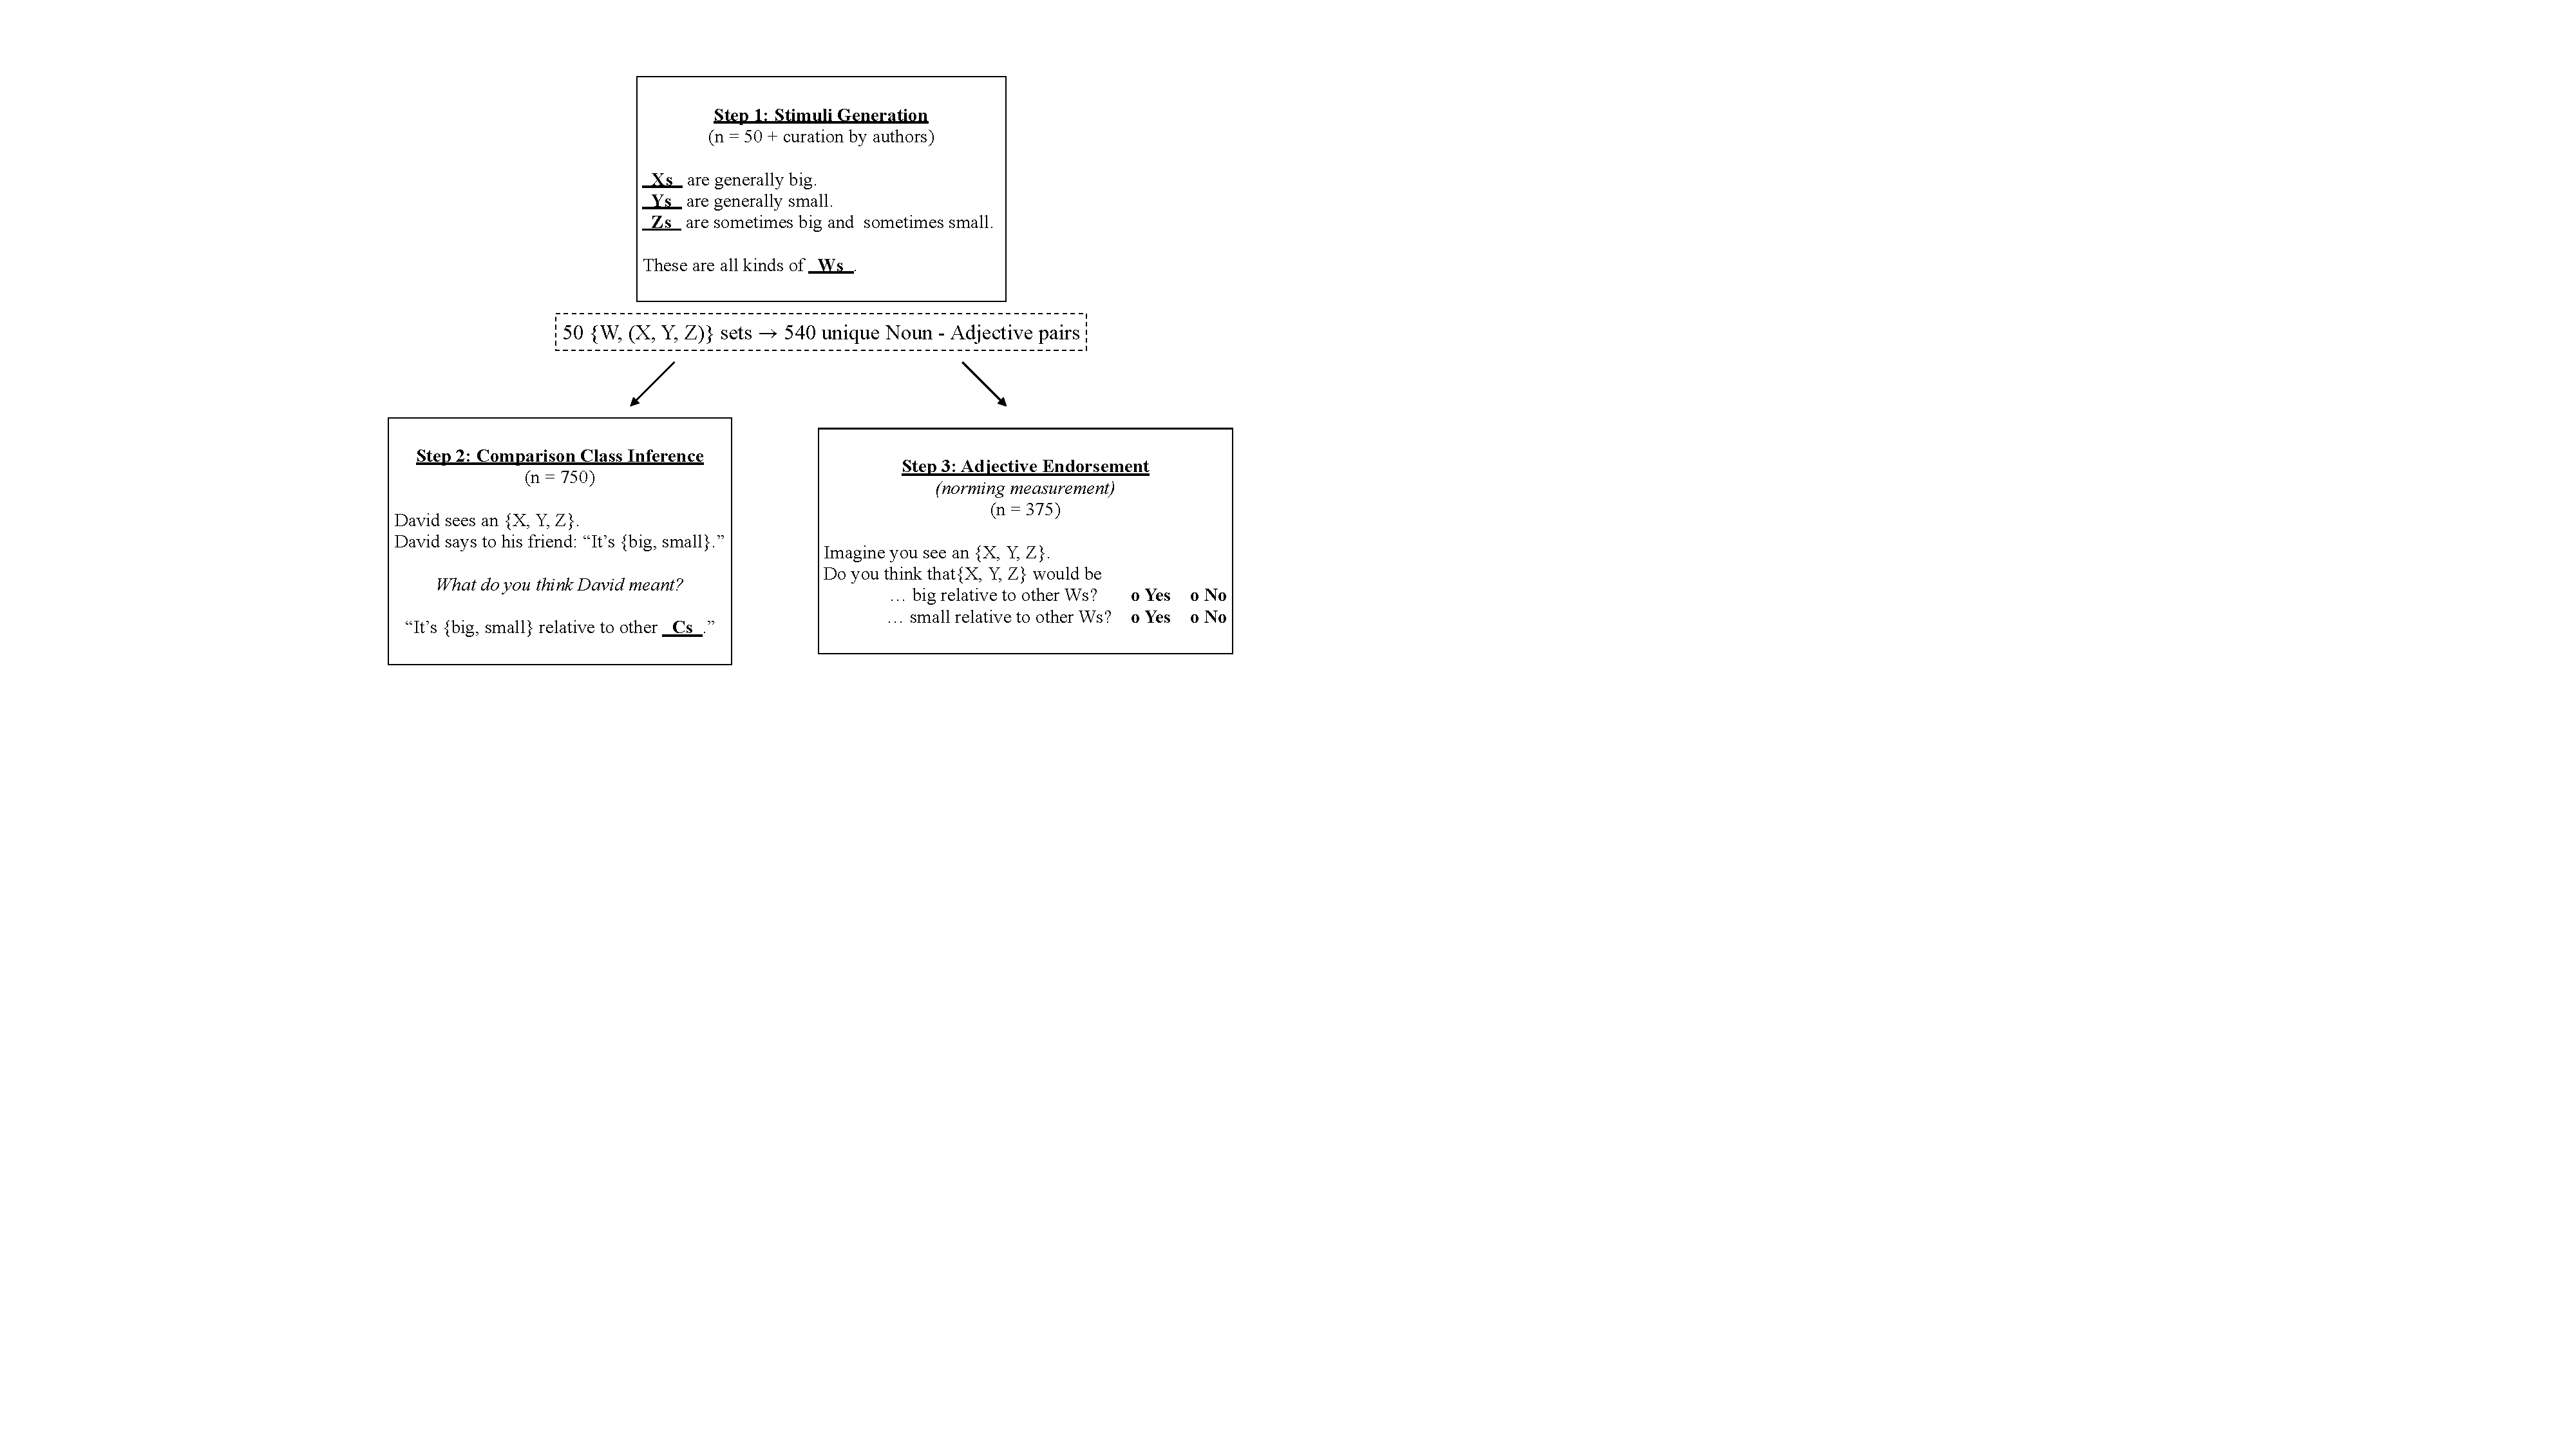
\includegraphics[width=0.9\textwidth]{figs/expt_overview} }
\caption{\small Overview of Experimental Tasks. Task 1: Using a structured production task, we elicit sets of stimuli that all share the feature of containing categories generally judged as having either a positive or negative adjective  (\emph{X, Y}; e.g., big or small) applied to them as well as a control category (\emph{Z}; e.g., sometimes big and sometimes small). The task is designed in a way to elicit three categories of the same basic- or superordinate-level category (\emph{W}). Task 2: Free-production task to elicit the comparison class. Task 3: Forced-choice task where participants judge whether a member of the subordinate level category would be judged as a having the adjective applied explicitly relative to the basic/superordinate level category. This task serves to provide additional data to constrain the parameters of the comparison class inference model. }\label{fig:exptOverview}
\end{figure*}


\subsection{Comparison Class Inference (Task 2)}

\subsubsection{Adaptive data collection procedure}

In this large set of items, we expected many items to have small variance in their judgments, requiring relatively fewer data points to estimate the probability of a subordinate~vs.~superordinate comparison class reliably.
We thus used a sequential sampling method on an item-wise basis, wherein we paused data collection after collecting 35 responses on each item.
We then analyzed the partial data set on a by-item basis to see which (if any) items had received exceedingly consistent responses, which we defined to be at least 33 out of 35  ($>94\%$ agreement) of the same response. 
For those items that received exceedingly consistent responses, we stopped data collection at 35 responses. This procedure allowed us to focus resources on providing better estimates for the items with more variability in responses. 
This adaptive procedure was decided ahead of time and is documented in the pre-registration report. 





\section{Bayesian Data Analysis}

The model's quantitative predictions can be generated by explicitly specifying the interlocutors' relevant prior knowledge (e.g., beliefs about temperatures). 
The current methodological standard is to measure prior beliefs empirically by creating tasks for participants to estimate quantities or give likelihood judgments \cite{Franke2016}. 
We pursue a different methodology. 
The RSA model captures a productive fragment of natural language; thus, it makes predictions about a related natural language task.
Critically, we can use the model to predict natural language judgments that require the \emph{same prior knowledge} as in Expt. 1 and use Bayesian data analysis to jointly infer the shared priors. 
This approach harnesses the productivity of language into experiment design and allows us to reconstruct priors without having participants engage in challenging numerical estimation tasks.

\subsection{Overview of data analytic approach}

The behavioral experiment bore out our two qualitative predictions
derived from the comparison class inference model. The model is a
quantitative model, however, and can make quantitative predictions
concerning the strength of comparison class inferences. Indeed, we
observe substantial variability in the predicted inferences both within-
and across- scales. Here we test whether the observed variability in
inferences can be accounted for by the constructs posited in our model.
We describe the two relevant constructs---the comparison class prior
\(P(c)\) and the degree priors \(P(x \mid c)\)---before outlining our
Bayesian data analytic strategy.

\subsubsection{Comparison class prior}

\(P(c)\) reflects listeners' expectations of what classes are likely to be discussed. As a proxy for comparison class usage frequency, we use empirical frequency \(\hat{f}\) estimated from the Google WebGram corpus\footnote{Corpus accessed via
\url{https://corpora.linguistik.uni-erlangen.de/cgi-bin/demos/Web1T5/Web1T5_freq.perl}. 
Due to potential polysemy and idiosyncracies of our experimental
  materials (Table 1), we made the following substitutions when querying
  the database for empirical frequency: produce $\rightarrow$
  ``fruits and vegetables''; things you watch online
  $\rightarrow$ ``online videos''; days in \{season\}
  $\rightarrow$ ``\{season\} days''; dishwashers $\rightarrow$
  ``dishwashing machines''; videos of cute animals $\rightarrow$
  ``animal videos''.}, and scale it by a free parameter $\beta$ such that $P(c) \propto \exp{(\beta \cdot \log \hat{f})}$.

\subsubsection{Degree priors (World knowledge)}

Only the relative values for \(P(x \mid c_{sub})\) and \(P(x \mid c_{super})\) affect model predictions. 
Hence we fix each superordinate distribution to be a standard normal distribution \(P(x \mid c_{super}) = \mathcal{N}(0, 1)\) and the subordinate priors to also be Gaussian distributions \(P(x \mid c_{sub}) = \mathcal{N}(\mu_{sub}, \sigma_{sub})\); the subordinate priors thus have standardized units.

Specifying the relevant prior knowledge yields two free parameters per subordinate class. We put priors over these parameters and infer their likely values using Bayesian data analysis. The data from the comparison class inference experiment would be insufficient, however, to reliably estimate all of the parameters of this data analytic model. To alleviate this, we use the same RSA model to predict additional data about related language used in the same domains. Specifically, we gather judgments about adjectives when the comparison class is explicit (\(n = 100\)): whether or not an adjective would apply to a subordinate member explicitly relative to the superordinate category (e.g., Is a day in winter warm relative to other days of the year?).\footnote{The judgments in this experiment were consistent with the \emph{a priori} ordering of the subordinate categories on the degree scale (e.g., a day in winter is likely to be cold for the year).}

To model this adjective endorsement data, we remove comparison class uncertainty by setting \(P(c_{super}) = 1\), since the sentence being endorsed include an explicit comparison to the superordinate class. We model sentence endorsement using a pragmatic speaker (following Qing \&Franke, 2014a; Tessler \& Goodman, 2016a, 2016b): \vspace{-0.5cm}
\begin{equation}
S_{2}(u \mid c_{sub}) \propto \exp{(\alpha_2 \cdot {\mathbb E}_{x\sim P_{c_{sub}}} \ln{L_1(x \mid u)})} \label{eq:S2a}
\end{equation} 

\noindent Note that $L_1(x \mid u)$ is defined from Eq. \ref{eq:L1a} by marginalization.

Eqs. \ref{eq:L1a} and \ref{eq:S2} define models for the comparison class inference task and adjective endorsement task, respectively, and depend on the same background knowledge \(P(x\mid c)\). We can thus use data from both experiments to jointly reconstruct the shared prior knowledge and generate predictions for the two data sets.

\section{Full model analysis and results}

The RSA listener (Eq. \ref{eq:L1a}) and speaker (Eq. \ref{eq:S2}) models make quantitative predictions about comparison class interpretation and adjective endorsement, respectively. We construct a single data-analytic model with each of these RSA components as sub-models in order to make quantitative predictions about the data from both of our experiments.

The listener and speaker sub-models share their prior world knowledge \(P(x \mid c)\) (e.g., temperatures in winter), described in the \textbf{Degree Priors} section. We put the same priors over the parameters of each subordinate distribution:
\(\mu \sim \text{Uniform}(-3, 3)\), \(\sigma \sim \text{Uniform}(0, 5)\), since they have standardized units. The comparison class prior \(P(c)\) in Eq. \ref{eq:L1a} scales the empirical frequency \(\hat{f}\) by a free parameter, which we give the following prior: \(\beta \sim \text{Uniform}(0, 3)\).

The full model has three additional parameters not of direct theoretical interest: the speaker optimality parameters \(\alpha^\text{expt}_{i}\), which can vary across the two tasks. The pragmatic listener \(L_1\) model (Eq. \ref{eq:L1a}) has one speaker optimality: \(\alpha^\text{1}_{1}\). The pragmatic speaker \(S_2\) model (Eq. \ref{eq:S2}) has two speaker optimality parameters: \(\{\alpha^\text{2}_{1}, \alpha^\text{2}_{2}\}\). We use priors consistent with the previous literature: \(\alpha_1 \sim \text{Uniform}(0, 20)\), \(\alpha_2 \sim \text{Uniform}(0, 5)\)

We implemented the RSA and Bayesian data analysis models in the probabilistic programming language WebPPL (Goodman \& Stuhlmuller, 2014). To learn about the credible values of the parameters, we collected 2 chains of 50k iterations (after 25k burn-in) using an incrementalized version of MCMC (Ritchie, Stuhlmuller, \& Goodman, 2016).

\subsubsection{Results}

The full model's posterior over the RSA and data-analytic parameters were consistent with prior literature and intuition. The maximum a-posteriori (MAP) estimate and 95\% highest probability density (HPD) intervals for model parameters specific to the \(L_1\) model used for comparison class inference were \(\alpha^{1}_{1} = 1.60 [1.10, 2.50]\),
\(\beta = 0.13 [0.11, 0.19]\). Model parameters specific to the \(S_2\) model used for adjective endorsement:
\(\alpha^{2}_{1} = 3.50 [0.60, 13.20]\), \(\alpha^{2}_{2} = 3.20 [2.60, 3.80]\). The inferred distributions corresponding to subordinate class priors were consistent with the \emph{a priori} ordering of these subordinate classes (low, medium, high) used in these tasks (Figure \ref{fig:modelParameters} top).

Finally, the full model's posterior predictive distribution does an excellent job at capturing the quantitative variability in comparison class inferences: \(r^2(30) = 0.96\), and adjective endorsements: \(r^2(30) = 0.98\) (Figure \ref{fig:posteriorPredictiveScatters}). Because of the overall preference for the subordinate comparison class, many of the data points are distributed above 0.5. Even for these fine-grained differences, the model does a good job at explaining the quantitative variability in participants' data (Figure \ref{fig:posteriorPredictiveScatters} right). Thus, the variability in comparison class inferences we observe in our behavioral data can be accounted for the constructs posited in our model (namely, the comparison class prior and degree priors).

\subsection{Fully Bayesian analysis of Bayesian language
models}

The second contribution of this paper is a novel data-analytic approach,
where prior knowledge used in the Bayesian language model is
reconstructed from converging evidence gathered from a related language
experiment, also explicitly modeled using a language understanding
model. In previous work, we have attempted to measure prior knowledge by
decomposing what would be a single, implicitly multilayered, numerical
estimation question into multiple simpler questions. Then, we construct
a Bayesian data analytic model to back out the prior knowledge (Tessler
\& Goodman, 2016a, 2016b). We extend this approach by using the same
core RSA model to model behavior across two language experiments. The
major feature of this method is that participants respond only to
simple, natural language questions rather than estimating numerical
quantities for which complicated linking functions must be designed
(e.g., Franke et al., 2016). The fully Bayesian language approach we
pioneer here also provides a further constraint on the language model,
which must predict data from two similar but distinct language
experiments. The productivity of natural language can thus be harnessed
to productively design experiments that further constrain and test
computational models of language and cognition.


\newpage


\bibliographystyle{apacite}

%\setlength{\bibleftmargin}{.125in}
%\setlength{\bibindent}{-\bibleftmargin}

\bibliography{comparison-class}

\end{document}
